% Options for packages loaded elsewhere
\PassOptionsToPackage{unicode}{hyperref}
\PassOptionsToPackage{hyphens}{url}
%
\documentclass[
]{book}
\usepackage{amsmath,amssymb}
\usepackage{iftex}
\ifPDFTeX
  \usepackage[T1]{fontenc}
  \usepackage[utf8]{inputenc}
  \usepackage{textcomp} % provide euro and other symbols
\else % if luatex or xetex
  \usepackage{unicode-math} % this also loads fontspec
  \defaultfontfeatures{Scale=MatchLowercase}
  \defaultfontfeatures[\rmfamily]{Ligatures=TeX,Scale=1}
\fi
\usepackage{lmodern}
\ifPDFTeX\else
  % xetex/luatex font selection
\fi
% Use upquote if available, for straight quotes in verbatim environments
\IfFileExists{upquote.sty}{\usepackage{upquote}}{}
\IfFileExists{microtype.sty}{% use microtype if available
  \usepackage[]{microtype}
  \UseMicrotypeSet[protrusion]{basicmath} % disable protrusion for tt fonts
}{}
\makeatletter
\@ifundefined{KOMAClassName}{% if non-KOMA class
  \IfFileExists{parskip.sty}{%
    \usepackage{parskip}
  }{% else
    \setlength{\parindent}{0pt}
    \setlength{\parskip}{6pt plus 2pt minus 1pt}}
}{% if KOMA class
  \KOMAoptions{parskip=half}}
\makeatother
\usepackage{xcolor}
\usepackage{color}
\usepackage{fancyvrb}
\newcommand{\VerbBar}{|}
\newcommand{\VERB}{\Verb[commandchars=\\\{\}]}
\DefineVerbatimEnvironment{Highlighting}{Verbatim}{commandchars=\\\{\}}
% Add ',fontsize=\small' for more characters per line
\usepackage{framed}
\definecolor{shadecolor}{RGB}{248,248,248}
\newenvironment{Shaded}{\begin{snugshade}}{\end{snugshade}}
\newcommand{\AlertTok}[1]{\textcolor[rgb]{0.94,0.16,0.16}{#1}}
\newcommand{\AnnotationTok}[1]{\textcolor[rgb]{0.56,0.35,0.01}{\textbf{\textit{#1}}}}
\newcommand{\AttributeTok}[1]{\textcolor[rgb]{0.13,0.29,0.53}{#1}}
\newcommand{\BaseNTok}[1]{\textcolor[rgb]{0.00,0.00,0.81}{#1}}
\newcommand{\BuiltInTok}[1]{#1}
\newcommand{\CharTok}[1]{\textcolor[rgb]{0.31,0.60,0.02}{#1}}
\newcommand{\CommentTok}[1]{\textcolor[rgb]{0.56,0.35,0.01}{\textit{#1}}}
\newcommand{\CommentVarTok}[1]{\textcolor[rgb]{0.56,0.35,0.01}{\textbf{\textit{#1}}}}
\newcommand{\ConstantTok}[1]{\textcolor[rgb]{0.56,0.35,0.01}{#1}}
\newcommand{\ControlFlowTok}[1]{\textcolor[rgb]{0.13,0.29,0.53}{\textbf{#1}}}
\newcommand{\DataTypeTok}[1]{\textcolor[rgb]{0.13,0.29,0.53}{#1}}
\newcommand{\DecValTok}[1]{\textcolor[rgb]{0.00,0.00,0.81}{#1}}
\newcommand{\DocumentationTok}[1]{\textcolor[rgb]{0.56,0.35,0.01}{\textbf{\textit{#1}}}}
\newcommand{\ErrorTok}[1]{\textcolor[rgb]{0.64,0.00,0.00}{\textbf{#1}}}
\newcommand{\ExtensionTok}[1]{#1}
\newcommand{\FloatTok}[1]{\textcolor[rgb]{0.00,0.00,0.81}{#1}}
\newcommand{\FunctionTok}[1]{\textcolor[rgb]{0.13,0.29,0.53}{\textbf{#1}}}
\newcommand{\ImportTok}[1]{#1}
\newcommand{\InformationTok}[1]{\textcolor[rgb]{0.56,0.35,0.01}{\textbf{\textit{#1}}}}
\newcommand{\KeywordTok}[1]{\textcolor[rgb]{0.13,0.29,0.53}{\textbf{#1}}}
\newcommand{\NormalTok}[1]{#1}
\newcommand{\OperatorTok}[1]{\textcolor[rgb]{0.81,0.36,0.00}{\textbf{#1}}}
\newcommand{\OtherTok}[1]{\textcolor[rgb]{0.56,0.35,0.01}{#1}}
\newcommand{\PreprocessorTok}[1]{\textcolor[rgb]{0.56,0.35,0.01}{\textit{#1}}}
\newcommand{\RegionMarkerTok}[1]{#1}
\newcommand{\SpecialCharTok}[1]{\textcolor[rgb]{0.81,0.36,0.00}{\textbf{#1}}}
\newcommand{\SpecialStringTok}[1]{\textcolor[rgb]{0.31,0.60,0.02}{#1}}
\newcommand{\StringTok}[1]{\textcolor[rgb]{0.31,0.60,0.02}{#1}}
\newcommand{\VariableTok}[1]{\textcolor[rgb]{0.00,0.00,0.00}{#1}}
\newcommand{\VerbatimStringTok}[1]{\textcolor[rgb]{0.31,0.60,0.02}{#1}}
\newcommand{\WarningTok}[1]{\textcolor[rgb]{0.56,0.35,0.01}{\textbf{\textit{#1}}}}
\usepackage{longtable,booktabs,array}
\usepackage{calc} % for calculating minipage widths
% Correct order of tables after \paragraph or \subparagraph
\usepackage{etoolbox}
\makeatletter
\patchcmd\longtable{\par}{\if@noskipsec\mbox{}\fi\par}{}{}
\makeatother
% Allow footnotes in longtable head/foot
\IfFileExists{footnotehyper.sty}{\usepackage{footnotehyper}}{\usepackage{footnote}}
\makesavenoteenv{longtable}
\usepackage{graphicx}
\makeatletter
\def\maxwidth{\ifdim\Gin@nat@width>\linewidth\linewidth\else\Gin@nat@width\fi}
\def\maxheight{\ifdim\Gin@nat@height>\textheight\textheight\else\Gin@nat@height\fi}
\makeatother
% Scale images if necessary, so that they will not overflow the page
% margins by default, and it is still possible to overwrite the defaults
% using explicit options in \includegraphics[width, height, ...]{}
\setkeys{Gin}{width=\maxwidth,height=\maxheight,keepaspectratio}
% Set default figure placement to htbp
\makeatletter
\def\fps@figure{htbp}
\makeatother
\setlength{\emergencystretch}{3em} % prevent overfull lines
\providecommand{\tightlist}{%
  \setlength{\itemsep}{0pt}\setlength{\parskip}{0pt}}
\setcounter{secnumdepth}{5}
\usepackage{booktabs}
\ifLuaTeX
  \usepackage{selnolig}  % disable illegal ligatures
\fi
\usepackage[]{natbib}
\bibliographystyle{plainnat}
\usepackage{bookmark}
\IfFileExists{xurl.sty}{\usepackage{xurl}}{} % add URL line breaks if available
\urlstyle{same}
\hypersetup{
  pdftitle={A Course on Advanced Regression Models, Causal Inference, and Data Visualization},
  pdfauthor={Christopher Weber},
  hidelinks,
  pdfcreator={LaTeX via pandoc}}

\title{A Course on Advanced Regression Models, Causal Inference, and Data Visualization}
\author{Christopher Weber}
\date{2024-08-26}

\begin{document}
\maketitle

{
\setcounter{tocdepth}{1}
\tableofcontents
}
\chapter*{}\label{section}
\addcontentsline{toc}{chapter}{}

\section*{Preface}\label{preface}
\addcontentsline{toc}{section}{Preface}

The purpose of this course is to introduce students to advanced techniques in regression, statistical computation, and techniques in scientific reproducibility and transparency. Students in this course should be very familiar with linear regression, as well as the Gauss-Markov assumptions underlying the classical linear model (i.e., POL 682). In this course, we will consider a variety of regression techniques for categorical and limited data. It is essential to remain up-to-date on the readings, as well as apply the reviewed methods to existing data.

The course will progress through several related sections. The first part will focus on several theoretical factors pertaining to statistical inference. We will start by considering two fundamental approaches underlying inference, the likelihood principle and Bayes' rule. We will also re-consider the linear model, the Gauss-Markov assumptions, and we will review several concepts and statistical distributions. In this section we will also consider the practical trade off researchers encounter pertaining to efficiency and bias.

In the second section, we will move to discrete dependent and limited variables. In practice, it is quite rare to encounter dependent variables that are continuous and normally distributed. In circumstances with binary, ordinal, and other multicategory dependent variables, the Gauss-Markov assumptions will be violated, thus rendering OLS an inappropriate choice. At this juncture, we will use both maximum likelihood (ML) and Bayesian methods to estimate logit, probit, multinomial logit/probit, and ordinal logit/probit models.

Political scientists often encounter datasets that involve event counts (e.g., war casualties, number of conflict events, elections won by a candidate). These variables rarely follow a normal distribution; instead, they are heavily skewed. After the logit/probit weeks, we'll consider several type of count-oriented regression models, including the Poisson, Negative Binomial, and ``Hurdle'' models. We will then transition to censored and sample selection models.

In the final section, we will consider a variety of topics that extend the models from the previous weeks. For instance, ``endogeneity'' is a common problem to arise in applied settings -- an independent variable is correlated with the error term. We'll look this problem in several ways, followed with several common solutions. We will examine two-stage least squares, three-stage least squares, and matching methods.Finally, we will examine hierarchical models.

Three major points need to be emphasized. First, many of the statistical methods build on models discussed in previous weeks. It is essential to keep up-to-date on readings, and if there is something that confuses you, please see me as soon as possible. Second, I find that the best way to learn these techniques is to implement them. I strongly recommend you find a dataset and work with this dataset throughout the semester. Even if your analysis is not always substantively interesting, at the very least, you will have the code for future use. Third, I strongly encourage you to give yourself sufficient time to complete the course requirements. One of the worst ways to learn statistics is through cramming and completing assignments at the very last minute. As you likely know, I am flexible with due dates and generally accept late assignments. Don't take advantage of this policy! Handing things in late and consistently placing other obligations before this class has the potential to adversely impact what you learn.

\chapter{Syllabus}\label{syllabus}

\section*{POL 683: Advanced Regression Analysis}\label{pol-683-advanced-regression-analysis}
\addcontentsline{toc}{section}{POL 683: Advanced Regression Analysis}

\subsection*{Fall 2024}\label{fall-2024}
\addcontentsline{toc}{subsection}{Fall 2024}

Tuesdays 9:00PM - 11:30AM

\textbf{Instructor:}

Christopher Weber, PhD

School of Government and Public Policy

University of Arizona 333

Social Sciences Building

\href{mailto:chrisweber@arizona.edu}{\nolinkurl{chrisweber@arizona.edu}}

Office Hours: T 12:00PM-1:30PM (and by appointment).

\section{Course Description}\label{course-description}

The purpose of this course is to introduce students to advanced techniques in regression, statistical computation, and techniques in scientific reproducibility and transparency. Students in this course should be very familiar with linear regression, as well as the Gauss-Markov assumptions underlying the classical linear model (i.e., POL 682). In this course, we will consider a variety of regression techniques for categorical and limited data. It is essential to remain up-to-date on the readings, as well as apply the reviewed methods to existing data.

The course will progress through several related sections. The first part will focus on several theoretical factors pertaining to statistical inference. We will start by considering two fundamental approaches underlying inference, the likelihood principle and Bayes' rule. We will also re-consider the linear model, the Gauss-Markov assumptions, and we will review several concepts and statistical distributions. In this section we will also consider the practical trade off researchers encounter pertaining to efficiency and bias.

In the second section, we will move to discrete dependent and limited variables. In practice, it is quite rare to encounter dependent variables that are continuous and normally distributed. In circumstances with binary, ordinal, and other multicategory dependent variables, the Gauss-Markov assumptions will be violated, thus rendering OLS an inappropriate choice. At this juncture, we will use both maximum likelihood (ML) and Bayesian methods to estimate logit, probit, multinomial logit/probit, and ordinal logit/probit models.

Political scientists often encounter datasets that involve event counts (e.g., war casualties, number of conflict events, elections won by a candidate). These variables rarely follow a normal distribution; instead, they are heavily skewed. After the logit/probit weeks, we'll consider several type of count-oriented regression models, including the Poisson, Negative Binomial, and ``Hurdle'' models. We will then transition to censored and sample selection models.

In the final section, we will consider a variety of topics that extend the models from the previous weeks. For instance, ``endogeneity'' is a common problem to arise in applied settings -- an independent variable is correlated with the error term. We'll look this problem in several ways, followed with several common solutions. We will examine two-stage least squares, three-stage least squares, and matching methods.Finally, we will examine hierarchical models.

Three major points need to be emphasized. First, many of the statistical methods build on models discussed in previous weeks. It is essential to keep up-to-date on readings, and if there is something that confuses you, please see me as soon as possible. Second, I find that the best way to learn these techniques is to implement them. I strongly recommend you find a dataset and work with this dataset throughout the semester. Even if your analysis is not always substantively interesting, at the very least, you will have the code for future use. Third, I strongly encourage you to give yourself sufficient time to complete the course requirements. One of the worst ways to learn statistics is through cramming and completing assignments at the very last minute. As you likely know, I am flexible with due dates and generally accept late assignments. Don't take advantage of this policy! Handing things in late and consistently placing other obligations before this class has the potential to adversely impact what you learn.

\section{Learning Objectives}\label{learning-objectives}

In this class, students will complete the following.

\begin{itemize}
\item
  Identify the tools involved in advanced regression analysis.
\item
  Use these methods in applied settings.
\item
  Understand the appropriate regression analysis in various settings.
\end{itemize}

\emph{Required Course Readings}

Long, J. Scott. 1997. \emph{Regression Models for Categorical and Limited Dependent Variables}. Sage: New York.

McElreath, Richard 2020. Statistical Rethinking: A Bayesian Course with Examples in Stan and R.Cambridge: Cambridge University Press.

Additional Required Readings

I have assigned a number of journal articles, which may be accessed through the University of Arizona Library. They are all available for download through JSTOR and/or e-journals.

\emph{Recommended Readings}

Eliason, Scott. 1993. Maximum Likelihood Estimation: Logic and Practice. Thousand Oaks, CA: Sage.

Fox, John. 2008. Applied Regression Analysis and Generalized Linear Models, Second Edition. Thousand Oaks, California: Sage.

Gelman, Andrew, John Carlin, Hal Stern, David Dunson, Aki Vehtari, and Donald Rubin. 2014. Bayesian Data Analysis, Third Edition. CRC Press: New York.

King, Gary. 1998. Unifying Political Methodology: The Likelihood Theory of Statistical Inference. Michigan University Press: Ann Arbor.

Berry, William and Stanley Feldman. 1985 Multiple Regression In Practice. Newbury, CA: Sage.

Gelman, Andrew and Jennifer Hill. 2007.Data Analysis Using Regression and Multilevel/Hierarchical Models. Cambridge: Cambridge University Press.

William H. Greene. Econometric Analysis, 8th Edition. New York: Pearson. (From 682)

\textbf{Statistical Software}

There are many statistical software packages available, all of which will perform the functions explored in this class. We will be relying on \emph{R}, a free statistical program available for Mac, Windows, and Linux. R may be downloaded from the CRAN website (\url{http://www.r-project.org}). The CRAN site also includes a variety of user's manuals, which I suggest you consult early in the semester (if you are unfamiliar with the R language).

We will explore a variety of Rfunctions throughout the semester. I will assume that you know the ``basics,'' such as opening a dataset, accessing variables, and creating new variables. I will also assume that you can run and estimate simple linear regression models, manipulate/recode data, and access saved objects.

We will also rely heavily on the \textbf{\emph{Stan}} language for Bayesian models. Stan can be run on a variety of platforms; I would recommend using R. Please follow the instructions on this page:

\href{https://github.com/stan-dev/rstan/wiki/RStan-Getting-Started}{\emph{https://github.com/stan-dev/rstan/wiki/RStan-Getting-Started}}

Also, download and start following the Stan User's Manual:

\href{http://mc-stan.org/documentation/}{\emph{http://mc-stan.org/documentation/}}

I strongly recommend you install Stan in the first week of the semester. Occasionally, problems arise. These should be addressed early in the semester.

There is a really easy-to-use package in R called brms. We'll use it throughout the term -- it follows the structure of a \emph{lm} call, but compiles and runs a stan regression model.

\emph{Open Science}

This class strives to advance an open science framework, a shift in the basic and social sciences to make research, data, code, and publications open and accessible. In this class, we will discuss scientific techniques that promote collaboration, transparency, and reproducibility. This means we will generally rely on free tools -- like R -- public repositories and develop research protocols that are transparent and well documented. In practice, this means:

\begin{itemize}
\item
  We will regularly use open source software, like R.
\item
  We will develop open source code, by posting code on Github.
\item
  We will generate modular computer code.
\item
  We will generate code that produces reproducible examples.
\item
  We will generate clear clear documentation.
\item
  In addition to a variety of packages in R, we will rely on one built for this class (and very much, in production). It is called \textbf{advancedRegression}. You will periodically need to re-install package, as we'll make updates through the semester.
\end{itemize}

\textbf{Collaboration}. I tend to find that the most useful way to learn statistics is to practice statistics. I suspect this class will be far easier if you take the time (i.e., a few hours every week) to implement the procedures we discuss in class. I will make most of my code for this class available through github. We'll spend some time on basic github operations in this cousre, so there is no need to set up anything in advance (simply be sure you have a github acct.)

\textbf{Github} is a tool for version control and collaboration. You should create agithub user account during the first week, in addition to acquainting yourself with the service. Please also read some of the online tutorials regarding github and how to set it up with Rstudio orR. If you use an email other than your University of Arizona email, please let me know.

\emph{Important Information }

If you feel sick, or may have been in contact with someone who is infectious, stay home. Except for seeking medical care, avoid contact with others and do not travel.

The UA policy regarding absences on and accommodation of religious holidays is available here: (\url{http://deanofstudents.arizona.edu/religiousobservanceandpractice}. Visit the UArizona COVID-19 page for regular updates.

Life challenges: If you are experiencing unexpected barriers to your success in your courses, please note the Dean of Students Office is a central support resource for all students and may be helpful. The Dean of Students Office can be reached at 520-621-2057 or \href{mailto:DOS-deanofstudents@email.arizona.edu}{\nolinkurl{DOS-deanofstudents@email.arizona.edu}}.

Physical and mental-health challenges: If you are facing physical or mental health challenges this semester, please note that Campus Health provides quality medical and mental health care. For medical appointments, call (520-621-9202. For After Hours care, call (520) 570-7898. For the Counseling and Psych Services (CAPS) 24/7 hotline, call (520) 621-3334.

Equipment and software requirements: For this class you will need daily access to the following hardware: laptop or web-enabled device with webcam and microphone; regular access to reliable internet signal; ability to download and run the following software: R/RStudio. You should install rstan, tidy, dplyr, ggplot2, pscl, and nnet packages within the first week of the course.

Staying current: You are required to complete course assignments by the due date.

Students who turn in an assignment on the due date but after the beginning of class will lose a minimum of one letter grade. An additional letter grade will be deducted for each day the assignment is late. Depending on where we are in the class, I may decide to alter a due date. Any changes will be announced in classes. Makeup exams or assignments will be allowed only in the case of university excused absences. Again, documentation must be provided.

Threatening behavior is unacceptable and will be reported. The Arizona Board of Regents' Student Code of Conduct, ABOR Policy 5-308, prohibits threats of physical harm to any member of the University community, including to one's self. See: \url{http://policy.arizona.edu/threatening-behavior-students}.

It is the University's goal that learning experiences be as accessible as possible. If you anticipate or experience physical or academic barriers based on disability, please let me know immediately so that we can discuss options. You are also welcome to contact Disability Resources (520-621-3268) to establish reasonable accommodations. Please be aware that the accessible table and chairs in this room should remain available for students who find that standard classroom seating is not usable.

It is your responsibility to complete all works assigned in this course (e.g., tests, assignments) in full observation of the Student Code of Academic Integrity. Students are encouraged to share intellectual views and discuss freely the principles and applications of course materials. However, graded work/exercises must be the product of independent effort unless otherwise instructed. Students are expected to adhere to the UA Code of Academic Integrity as described in the UA General Catalog. See: \url{http://deanofstudents.arizona.edu/codeofacademicintegrity}.

In addition, the University Libraries have some excellent tips for avoiding plagiarism available at: \href{http:///url\%7Bwww.library.arizona.edu/help/tutorials/plagiarism/index.html}{www.library.arizona.edu/help/tutorials/plagiarism/index.html}.

According to Section D (6) (a) of the University's Intellectual Property Policy (which is available at \url{http://www.ott.arizona.edu/uploads/ip_policy.pdf}. faculty own the intellectual property for their course notes and course materials. The instructor holds the copyright to his/her lectures and course materials, including student notes or summaries that substantially reflect them. Student notes and course recordings are for individual use or for shared use on an individual basis. Selling class notes and/or other course materials to other students or to a third party for resale is not permitted without the instructor's express written consent. Violations to the instructor's copyright are subject to the Code of Academic Integrity and may result in course sanctions. Additionally, students who use D2L or UA email to sell or buy these copyrighted materials are subject to Code of Conduct Violations for misuse of student email addresses.

For more information on the confidentiality of student records, please see \url{http://www.registrar.arizona.edu/ferpa/default.htm}

\(\bullet\) Requests for incompletes (I) and withdrawal (W) must be made in accordance with university policies which are available at \url{http://catalog.arizona.edu/2012-13/policies/grade.htm\#I} and \url{http://catalog.arizona.edu/2012-13/policies/grade.htm\#W}, respectively.

\(\bullet\) The UA's policy concerning Class Attendance and Administrative Drops is available at: \url{http://catalog.arizona.edu/2012-13/policies/classatten.htm}

\section{Grades}\label{grades}

90\%-100\% A

80\%-89\% B

70\%-79\% C

60\%-69\% D

59\% and below E

\textbf{Graded Items}

\begin{longtable}[]{@{}
  >{\raggedright\arraybackslash}p{(\columnwidth - 4\tabcolsep) * \real{0.1700}}
  >{\raggedright\arraybackslash}p{(\columnwidth - 4\tabcolsep) * \real{0.5500}}
  >{\raggedright\arraybackslash}p{(\columnwidth - 4\tabcolsep) * \real{0.2800}}@{}}
\caption{\textbf{Description of Graded Items.} Written projects comprise 40\% percent of your grade. For both the midterm and the final project, you will apply the techniques from this class to an actual data. The midterm paper consists of a challenge -- forecast the 2024 presidential election. Parts of this assignment will be done individually, other parts will be group work.}\tabularnewline
\toprule\noalign{}
\begin{minipage}[b]{\linewidth}\raggedright
\textbf{Component}
\end{minipage} & \begin{minipage}[b]{\linewidth}\raggedright
\textbf{Description}
\end{minipage} & \begin{minipage}[b]{\linewidth}\raggedright
\textbf{Percent of Final Grade}
\end{minipage} \\
\midrule\noalign{}
\endfirsthead
\toprule\noalign{}
\begin{minipage}[b]{\linewidth}\raggedright
\textbf{Component}
\end{minipage} & \begin{minipage}[b]{\linewidth}\raggedright
\textbf{Description}
\end{minipage} & \begin{minipage}[b]{\linewidth}\raggedright
\textbf{Percent of Final Grade}
\end{minipage} \\
\midrule\noalign{}
\endhead
\bottomrule\noalign{}
\endlastfoot
Midterm Project & Election forecast, short assignments and final report & 15\% \\
Midterm Exam & Short Answer/Problems & 25\% \\
Final Exam & Short Answer/Problems & 30\% \\
Final Paper & & 30\% \\
\end{longtable}

We will collaborate, but each person will play a unique role interpreting the results, which will form the basis for your grade. The goal for us, the challenge: \textbf{Create statistically informed set of predictions, effectively visualize these predictions, and finally, put the report on a public website.}

How will we do this? First, start by familiarizing yourself with:

\begin{itemize}
\item
  \textbf{Shiny}. Shiny is an open-source R package. It allows one to build interactive visualizations. This can be really important in academic work, as well as data science applications more generally. This book is a good resource, \hyperref[0]{https://mastering-shiny.org/}. And the documentation on the shiny website is also quite helpful, with many example \hyperref[0]{https://shiny.posit.co/r/gallery/}
\item
  \textbf{Github.} Code for the project should be pushed to the class repo.

  \textbf{crweber9874/advanced\_regression}

  \textbf{Data sources.} It is imperative that you research how others have generated election predictions, and where to find data. Should one use historical data, economic data, polling data, lots of polling data, and so forth? The project will entail a considerable amount of work, so it's important to regularly work on the project, rather than procrastinating until shortly before the due date.
\end{itemize}

\textbf{Protocol for Electoral Forecasting Project}

Please adhere to the following due dates.

\begin{itemize}
\item
  August 27, 2024: Create two research groups.
\item
  September 10, 2024: Generate model ideas.
\item
  October 1, 2024: Submit cleaned data, code, and documentation.
\item
  October 22: Submit predictions and brief report.
\item
  October 29: Build shiny application
\end{itemize}

You must also complete a final project. This should include an analysis using methods from this class -- i.e., the regression techniques from this class. The final paper should be between 10-15 pages in length. It is up to you to locate a dataset for both papers! I recommend exploring data options early in the semester, by searching for data on the ICPSR, Dataverse, or other data repositories. Alternatively, you are welcome to use data you have collected. You are free to choose the topic, but you must be able to provide me with the data used in your report. Again, your code should be shared on GitHub. If you or your advisor has proprietary data which I cannot access, you should not use this. I must be able to verify that you did all the necessary calculations honestly and accurately, which requires me being able to access any data you use. Also, if you rely on your own data, you must adhere to the University of Arizona's Institutional Review Board requirements.

The paper should include all the elements of a research paper. That said, my primary interest rests in your analyses. I ask that you be quite thorough when presenting the results. It is not sufficient to just run a regression and present the point estimates. Your paper should include detailed interpretation, robustness checks, and post-estimation clarification (which often come in the form of graphics). It should be a high quality paper; if you would not be comfortable presenting it at a conference, you should not feel comfortable handing it in for a grade. \emph{Do not just cut and paste R output. Tables and figures should be presented in a professional manner. I will deduct points for cut-and-pasted output from R.}

Your statistical models should be theoretically informed. I do not require a full-fledged introduction/literature review, though you should spend a page or two briefly describing the relevant literature. It is essential to include the formal hypotheses you will test, which should relate to this one/two page review. I will need to verify that your empirical tests match your expectations. Please follow American Psychological Association (APA) style or American Journal of Political Science (AJPS) style. The references should appear at the end of your manuscript. Please do not place the references in footnotes.

I strongly recommend you meeting with me periodically throughout the semester to discuss these projects.

There will be a midterm exam (25\%) and a final exam (30\%). The final will be cumulative, and will cover all material from the semester. The midterm and final should be completed in-class. You may use your notes and the course materials to complete the both exams. The exam must be completed independently.

\textbf{Important Due Dates for Graded Material}

Please adhere to the following due dates.

\begin{itemize}
\item
  August 27, 2024: Create two research groups (midterm project).
\item
  September 10, 2024: Model assignment (midterm project).
\item
  October 1, 2024: Submit cleaned data, code, and documentation (midterm project).
\item
  October 22: Submit predictions and brief report (midterm project).
\item
  November 5: Midterm Exam (in-class).
\item
  December 17: Final Exam (in-class).
\item
  December 17: Final Project. Please upload here
\end{itemize}

\url{https://arizona.box.com/s/snd55jtnk3iyygzgi8k3of0v5eq8fr7i}.

\section{Course Outline}\label{course-outline}

Please read all assigned readings prior to the listed meeting times. Please note that the course schedule is subject to change at my discretion. You are responsible for announced changes.

\emph{Key}

\(\bullet\) indicates a required reading

\(\rightarrow\) indicates a recommended reading

\(\star\) indicates an assignment.

\(\cdot\) indicates midterm project topic

Week 1 (8/27): Introduction

\(\bullet\) Long, Chapter 1.

\(\bullet\) McElreath, Chapter 1

\(\cdot\) Organize into small groups

Week 2 (9/3): Introduction to Maximum Likelihood and the Generalized Linear Model, I

\(\bullet\) Long, Chapter 2.

\(\bullet\) McElreath, Chapter 2

\(\rightarrow\) Gelman and Hill, Chapters 3 and 4.

\(\cdot\) Discuss data and model ideas.

\(\star\) \textbf{Models}. For next week, please bring model ideas to class. How should we predict election outcomes? What data should we use? Please write a brief (1-2 page) report listing ideas, perhaps elaborating on what others have done. There is no need for a formal literature review, but outlining the state of forecasting would be useful.

Week 3 (9/10): Introduction to Maximum Likelihood and the Generalized Linear Model, II

\(\bullet\) Long, Chapter 3.

\(\bullet\) McElreath, Chapter 3

\(\rightarrow\) Eliason, Scott R. 1993. Maximum Likelihood Estimation: Logic and Practice. Sage Monographs.

\(\rightarrow\) Fox, John. 2008. Applied Regression Analysis and Generalized Linear Models, Second Edition. Sage: New York. Chapter 15.

\(\cdot\) Discuss data and model ideas.

\subsection{Building a Statistical Model}\label{building-a-statistical-model}

Week 4 (9/17): Building a Model

\(\bullet\) McElreath, Chapter 4, and (pp.~323 - 345)

\(\bullet\) Freedman, Paul, Michael Franz, and Kenneth Goldstein. 2004. ``Campaign Advertising and Democratic Citizenship.'' American Journal of Political Science, 48(4): 723-741.

\(\bullet\) King, Gary and Langche Zeng. 2001. ``Logistic Regression in Rare Events Data.'' Political Analysis, 9(2): 137-173.

\(\rightarrow\) John Fox. 2008. Applied Regression Analysis and Generalized Linear Models, Second Edition. Sage: New York. Chapter 14.

\(\rightarrow\) King, Chapters 5, 6.

\(\cdot\) Discuss data and model ideas.

\(\star\) \textbf{Model} \textbf{Strategy}. As a group, develop a plan to generate electoral predictions. What are the strengths and weaknesses of your approach. Each group should meet outside of regular class time and draft a 1-2 page report for next week.

\subsection{Estimation and Model Fit}\label{estimation-and-model-fit}

Week 5 (9/24): Estimation, Prediction, Simulation

\(\bullet\) McElreath, Chapter 5

\(\bullet\) King, Gary, Michael Tomz and Jason Wittenberg. 2000. ``Making the Most of Statistical Analyses: Improving Estimation and Interpretation.'' American Journal of Political Science 44(2): 341-355.

\(\bullet\) Greenhill, Brian, Michael Ward, and Audrey Sacks. 2011. ``The Separation Plot: A New Visual Method for Evaluating the Fit of Binary Models.'' American Journal of Political Science, 55(4): 991-1002.

\(\bullet\) Herron, Michael. 2000. ``Post Estimation Uncertainty in Limited Dependent Variable Models.'' Political Analysis, 8(1): 83-98.

\(\cdot\) Discuss data, code, and reproducibility

\(\star\) \textbf{Data}. As a group, prepare data. Clean these data, prepare them for distribution, and write clear documentation.

\textbf{Simulation based approaches}

Week 6 (10/1): Introduction to Causal Inference and the Directed Acyclic Graph (DAG)

\(\bullet\) McElreath, Chapter 6

\(\bullet\) Jackman, Simon. 2000. ``Estimation and Inference via Bayesian Simulation: An Introduction to Markov-Chain Monte Carlo.'' American Journal of Political Science, 44(2): 375-404.

\(\bullet\) Western, Bruce and Simon Jackman. 1994. ``Bayesian Inference for Comparative Research.'' American Political Science Review, 88(2): 412-423.

\(\bullet\) Adrian Raftery. 1995. ``Bayesian Model Selection in Social Research.'' Sociological Methodology, 25, 111-163.

\(\rightarrow\) Stan User's Manual, Chapter 6.

\(\rightarrow\) Fox, John. 2008. Applied Regression Analysis and Generalized Linear Models, Second Edition. Sage: New York. Chapter 22.\textbackslash{}

\(\cdot\) Introduction to Shiny

\(\star\) \textbackslash textbf\{Midterm Project. Generate predictions, absolutely no later than 10/22. Each group should submit a csv file with the following headers: \textbackslash textbf\{state, \textbackslash textbf\{republican\textbackslash\_vote\textbackslash\_share\textbackslash\_prediction, \textbackslash textbf\{democratic\textbackslash\_vote\textbackslash\_share\textbackslash\_prediction. Thus will be three files -- two student groups, and my own. One 10/29, we'll build a Shiny app. Each group should also provide a 1-2 page report describing their statistical method, and perhaps walking the reader through code. Perhaps use R Markdown.

Models with Multi-category Discrete Variables

Week 7 (10/8): Multicategory models

\(\bullet\) Long, Chapters 5 and 6

\(\bullet\) McElreath, pp.~359 - 368

\(\bullet\) Alvarez, Michael and Jonathan Nagler. 1998. ``When Politics and Models Collide: Estimating Models of Multiparty Elections.'' American Journal of Political Science, 42(1): 55-96.

Count Data

Week 8 (10/15):

\(\bullet\) Long, Chapter 8.

\(\bullet\) McElreath, pp.~345-359; pp.~369-380

\(\bullet\) King, Gary. 1988. ``Statistical Models for Political Science Event Counts: Bias in Conventional Procedures and Evidence for the Exponential Poisson Regression Model.'' American Journal of Political Science, 32(3): 838-863.

Week 9 (10/22): Poisson, Overdispersion, and Underdispersion

\(\bullet\) McElreath, pp.~369-380

\(\bullet\) Wilson, Matthew and James Piazza. 2013. ``Autocracies and Terrorism: Conditioning Effects of Authoritarian Regime Type on Terrorist Attacks.'' American Journal of Political Science, 57(4): 941-955.

\(\bullet\) Box-Steffensmeier, Janet M., and Bradford S. Jones. 1997. ``Time is of the Essence: Event History Models in Political Science.'' American Journal of Political Science, 41(4): 1414-1461.

\textbackslash textbf\{Censored Data and Selection Bias

Week 10 (10/29): Censoring, Selection Bias

\(\bullet\) Long, Chapter 7.

\(\bullet\) Goren, Paul, Christopher Federico and Miki Caul Kittilson. 2009. ``Source Cues, Partisan Identities, and Political Value Expression.'' American Journal of Political Science, 53(4): 805-820.

\(\bullet\) Boehmke, Frederic, Daniel Morey, and Megan Shannon. 2006. ``Selection Bias and Continuous-Time Duration Models: Consequences and Proposed Solutions.'' American Journal of Political Science, 50(1): 192-207.

Week 11 (11/5): Midterm Exam

\textbf{Midterm Exam.} You may use notes and/or the textbook, though no computers, tablets, or phones may be used. (Frankly, AI does a great job answering my questions, and I need to protect the integrity of the exam). The exception is your phone can be used as a calculator.

Multilevel Data Structures.

Week 12 (11/12): Multilevel Analysis

\(\bullet\) McElreath, Chapter 13

Week 13 (11/19): Multilevel Analysis, Continued

\(\bullet\) McElreath, Chapter 14.

\(\bullet\) Steenbergen, Marco and Bradford Jones. 2002. ``Modeling Multilevel Data Structures.'' American Journal Political Science, 46(1): 218-237.

\(\bullet\) Stegmuller, Daniel. 2014.''How Many Countries for Multilevel Modeling? A Comparison of Frequentist and Bayesian Approaches.''American Journal Political Science, 57(3): 748-761.

Regularization and Non-Linearity

Week 14 (11/26): The Ridge and Lasso Models

\(\bullet\) McElreath, Chapter 7

\(\bullet\) Please read Chapter 6 in An Introduction to Statistical Learning. This chapter can be downloaded for free here: \href{http://web.stanford.edu/~hastie/pub.htm}{http://web.stanford.edu/\textbackslash\textasciitilde hastie/pub.htm}

\(\bullet\) Please read Chapter 5 in The Elements of Statistical Learning, Chapter 5. This chapter can be downloaded for free here: \href{http://web.stanford.edu/~hastie/pub.htm}{http://web.stanford.edu/\textbackslash\textasciitilde hastie/pub.htm}

Week 15 (12/3):

\(\bullet\) Gelman and Hill, Chapter 20.

\(\bullet\) End of semester workshop.

Week 16 (12/11): Workshop

\(\star\) \textbf{Final} \textbf{Exam}. You may use notes and/or the textbook, though no computers, tablets, or phones may be used. (Frankly, AI does a great job answering my questions, and I need to protect the integrity of the exam). The exception is your phone can be used as a calculator. The exam will take place on Tuesday, 12/17 from 8-10AM

\(\star\) Paper II is due by 12/17, 5PM. Please upload to D2L folder; code should be uploaded to your personal github repository.

\textbf{Have a wonderful break}

\chapter{Introduction}\label{introduction}

\section{The Logic of Inference}\label{the-logic-of-inference}

This class involves much more than finding a model that is appropriate for a given data structure. In fact, we will continually be returning to two themes in inferential statistics, the \emph{frequentist} and *Bayesian traditions. In some circumstances, these two traditions will yield very similar results, though the interpretations vary. During these first two weeks, we'll consider these two perspectives from a theoretical vantage; throughout the rest of the term, we'll review techniques to use these perspectives in inference.

It's worthwhile to understand the motivating principles of these two approaches, prior to digging into technical content. Most likely, many of you have received training in the \emph{frequentist} tradition of probability, which is often credited to Jerzy Neyman, Karl Pearson and Sir Ronald Fisher. The logic here is quite simple: Probability refers to the frequency of an event occurring in a series of trials.

Frequentism is actually quite intuitive when applied to circumstances in which we can observe repeated trials. If you flip a coin, the probability of observing heads is 0.5. What does that mean? Flip the coin 10000 times and you should expect to observe heads 5000 times.

Or consider the classic example of rolling a die. The probability of rolling a 1 (or any number, with a fair die) is 1/6. This number is of limited value in predicting the outcome of a single roll. Instead, what it means is that in a series of trials, approximately 1/6 of those trials will yield a 1. We could ask a variant of a classic game of chance question, which is if we have 10 trials, and each trial involves rolling two dice,is it beneficial to bet that at least one of those trials will yield two 1's (see \url{https://en.wikipedia.org/wiki/Problem_of_points})? The probability of observing two ones is 1/6 \(\times\) 1/6 \(=\) 1/36. This implies that the rest of the sample space (i.e., not rolling two ones) is 35/36. Since the rolls are independent, then the probability that two ones are not observed in 10 trials is \((35/36)^{10}=0.75\) -- thus one should probably \emph{not} bet on ``snake eyes.''

\begin{Shaded}
\begin{Highlighting}[]
\CommentTok{\# Load necessary library}
\FunctionTok{library}\NormalTok{(ggplot2)}

\CommentTok{\# Always set seed for reproducibility}
\FunctionTok{set.seed}\NormalTok{(}\DecValTok{123}\NormalTok{) }

\CommentTok{\# Simulate draws}
\NormalTok{n\_draws }\OtherTok{\textless{}{-}} \DecValTok{10000}
\NormalTok{outcomes }\OtherTok{\textless{}{-}} \FunctionTok{sample}\NormalTok{(}\FunctionTok{c}\NormalTok{(}\StringTok{"H"}\NormalTok{, }\StringTok{"T"}\NormalTok{), }\AttributeTok{size =}\NormalTok{ n\_draws, }\AttributeTok{replace =} \ConstantTok{TRUE}\NormalTok{, }\AttributeTok{prob =} \FunctionTok{c}\NormalTok{(}\FloatTok{0.5}\NormalTok{, }\FloatTok{0.5}\NormalTok{))}

\CommentTok{\# Create a data frame for plotting}
\NormalTok{df }\OtherTok{\textless{}{-}} \FunctionTok{data.frame}\NormalTok{(}\AttributeTok{Outcome =}\NormalTok{ outcomes)}

\CommentTok{\# Plot the results}
\FunctionTok{ggplot}\NormalTok{(df, }\FunctionTok{aes}\NormalTok{(}\AttributeTok{x =}\NormalTok{ Outcome)) }\SpecialCharTok{+}
  \FunctionTok{geom\_bar}\NormalTok{() }\SpecialCharTok{+}
  \FunctionTok{labs}\NormalTok{(}\AttributeTok{title =} \StringTok{"Simulated Coin Flips"}\NormalTok{, }\AttributeTok{x =} \StringTok{"Outcome"}\NormalTok{, }\AttributeTok{y =} \StringTok{"Frequency"}\NormalTok{) }\SpecialCharTok{+} 
  \FunctionTok{theme\_minimal}\NormalTok{()}
\end{Highlighting}
\end{Shaded}

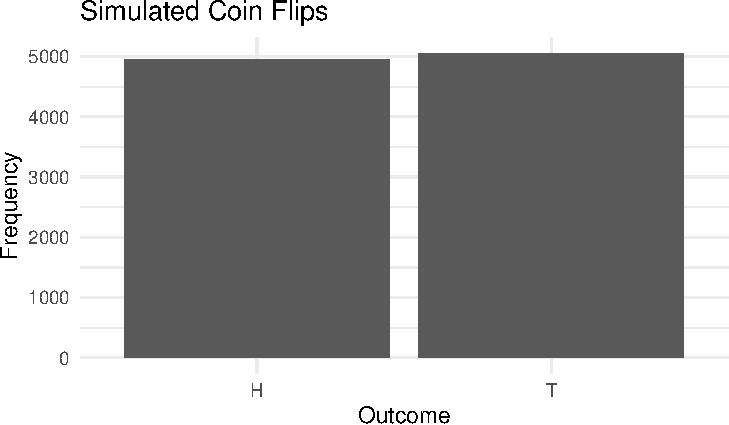
\includegraphics{_main_files/figure-latex/unnamed-chunk-2-1.pdf}

\begin{Shaded}
\begin{Highlighting}[]
\FunctionTok{paste}\NormalTok{(}\StringTok{"Of "}\NormalTok{, n\_draws, }\StringTok{" draws "}\NormalTok{,  }\FunctionTok{table}\NormalTok{(df)[}\DecValTok{1}\NormalTok{], }\StringTok{" were heads! "}\NormalTok{)}
\end{Highlighting}
\end{Shaded}

\begin{verbatim}
## [1] "Of  10000  draws  4943  were heads! "
\end{verbatim}

Be sure to set \emph{set.seed(10000)} to ensure reproducibility.

Statistics is often taught from this perspective -- even if not always clearly acknowledge. For instance, a confidence interval is not a statement of certainty regarding whether the derived interval contains the true population value. You were likely instructed, early on, that statements such as ``there's a 95\% chance the mean falls between and '\,' is incorrect. The reason is that frequentism hinges on the assumption that the population mean is fixed. If we were to repeatedly draw samples from a population and calculate a confidence interval, approximately 95\% of those intervals would capture the population value value.

In fact, the very logic of inference hinges on the notion of drawing a subset of the population (a sample) and making an inference about the general population from that sample. Yet, the \textbf{frequentist} approach forces us to think of the population parameter as fixed -- we simply don't have it because it would be expensive to collect -- and the methods we use to make inferences nearly always hinge on this notion of taking repeated samples from a population. Just recall the \textbf{central limit theore}, \textbf{the standard error}, \textbf{confidence intervals}, \textbf{p-values}, and \textbf{Type I} and \textbf{Type II} errors. These concepts all rely on the notion of repeated observation; hence, the frequentist'\,' label. Let's take a step back and consider what this means from the perspective of social science and sampling. Then, I think you'll see what I mean when I use the term \textbf{frequentist}.

\textbf{A Step Back}

In this class, and really in most everything you've worked on, the focus of the research is rarely on individual observations but rather distributions. We can summarize data, and relationships between variables, based on distributions. For example, recall that in linear regression, one of the assumptions is the error process follows a parametric distribution (often the normal distribution). Moreoever, if we have a dependent variable that is clearly not normal and continuous, then this assumption becomes tenuous.

Recall the differences between a probability density function (PDF) and a continuous density function (CDF). A PDF gives the probability of an occurence (for a discrete variable) or a range of occurences (for a continous variable).

\textbf{Notation}

\begin{enumerate}
\def\labelenumi{(\arabic{enumi})}
\item
  A CDF is written as F(x), or capital greek notation, e.g., \(\Gamma(x)\).
\item
  A PDF is written in lower case font, f(x), and we can find any area under a PDF by summation (for categorical data), and integration (for continuous data). That is,
\end{enumerate}

\[p(a<x<b)=\sum_i^{K} x_i\]

\[p(a<x<b)=\int f(x) dx\]

As such, \(F(\infty)=1\), and \(F(-\infty)=0\), and \(p(-\infty < x < \infty)=\int_{-\infty}^{\infty}f(x)dx=1\). This is an important principle, which occasionally is forgotten. The sum of the total under a probability distribution (continuous variable) or probability mass (discrete variable) must be 1. We can plot a distribution across \(x\) that displays the probabilities across values of \(x\). For a discrete distribution, the \(y\) axis represents the probability of observing discrete outcome \(x\); for a continuous outcome, the \(y\) axis represents a ratio, which is the probability of observing \(x\) within an (infinitesimally small) interval divided by the width of that interval. This ``density'' need not be 1 -- in fact, it's often not -- rather, the area under that distribution must be 1. Kruschke (2011) uses a nice analogy. Consider a sponge. The mass of the sponge represents the probability. Density is \(mass/volume\). If we squeeze the sponge, the mass doesn't change, though it's density clearly does. Here, volume, is simply the range of \(x\).

We should also be clear about notation. Oftentimes, we deal with two variables, \(x\) and \(y\). We'll often refer to things such as ``What is the probability of observing \(x\) averaged, or marginalized, across \(y\)?''

This is relatively easy to envision in a 2x2 table, in which we sum across rows or columns. The appropriate operation is then:

\[p(x)=\sum_y p(x_i, y_i) \hspace{0.5in}  \texttt{Marginal Probability}\]

Note, this only applies to a categorical distribution. Though, as we'll see, the continuous version is really just an extension of this.

Distributions are also used to describe continuous variables. In fact, much of the applications in this class will assume a continous distribution, even if we only observe a discrete response option. In your first semester statistics course, you reviewed the properties of a variety of continuous distributions -- I assume, the \textbf{normal}, \textbf{poisson}, \textbf{student's t}, \textbf{F}, and so forth. One can use univariate calculus -- integration, in particular -- to calculate various areas under the curve. If this is foreign to you, because you forgot it or didn't quite grasp the concept from your first semester class, I strongly recommend you go back and review this material. We cannot spend much time on reviewing the basics of integration, and we will use it frequently in this class. Back to the issue at hand. For a continuous bivariate density, then

\[p(x)=\int p(x, y) dy \hspace{0.5in}  \texttt{Marginal Probability}\]

Notice here the only difference is the \(\int\) instead of \(\sum\). But, it's useful to think of them as calling for the same thing. Then the \(dy\) simply means ``averaged across y.'' Sometimes we say that this operation entails \emph{integrating out y}, or \emph{averaging across y.}

There are also conditional probabilities; these are not the same as marginal probabilities. For instance, we might ask, ``what is the probability that a wrestler has died, given he/she is 35-40?'\,' So, \(p(X=(death) | Y=35-40)\). The conditional probability is always,

\[p(x|y)=p(x,y)/p(y)\hspace{0.5in}  \texttt{Conditional Probability}\]

where, \(p(x)=\sum_y p(x, y)\) or \(p(x)=\int p(x, y) dy\). In other words, we are taking the joint probability of two things happening, here \(p(x,y)\), and dividing the joint probability by the marginal probability of observing y, \(p(y)\). Think of it as the joint probability weighted by the marginal probability.

And, finally, we will almost always assume independence, such that the probability of one outcome does not depend on the probability of a second outcome. In a bivariate distribution, this means

\[p(x,y)=p(x) p(y) \hspace{0.5in}  \texttt{Independence}\]

This is actually quite intuitive if you think about it. If \(p(x)\) and \(p(y)\) are entirely unrelated -- knowing one does not help you know the other -- then the probability of observing the two events is simply the product. If I flip a coin from 1989 and one from 1977, the flips are independent. Knowing the outcome of the 1989 coin flip is inconsequential for the outcome of the 1977 coin flip. By extension, if two events are independent, then the conditional probability \(p(x|y)=p(x)\). Think briefly about what this means in context of the coin flip. Given that the Canadian coins is head, what is the probability that the 1989 coin is heads?

We can extend these ideas further, leveraging these three basic principles to what is known as \textbf{Bayes' Rule}, named after the mathematician Reverand Thomas Bayes.

\section{Conditional Probabilities, Continued: Bayes' Rule}\label{conditional-probabilities-continued-bayes-rule}

Consider the probability of observing \(x\) given \(y\). This probability can be expressed as the joint probability of observing \(x\) and \(y\) divided by the marginal probability of observing \(y\). That is,

\[p(x|y)=p(x,y)/p(y)\]

We can just rearrange things to find \(p(y|x)\). First multiply the equation by \(p(y)\)

\[p(x|y) p(y)=p(x,y) \]

But, remember, we can find the joint probability, \(p(x,y)\) as

\[p(y|x) p(x)=p(y,x) \]

Meaning,

\[p(x|y) p(y)=p(y|x) p(x)\]

Bayes' Rule is simply,

\[p(y|x) =[p(x|y) p(y)]/p(x)\]

Notice, that we could simply solve this by inverting the rows and columns in the above example.

We'll rely heavily on this basic principle, extending it in a number of interesting ways. For now, it's more than sufficient to simply understand that Bayes' Rule is really just a reordering of what we know about conditional probabilities.

\textbf{Why p(y\textbar x) is important -- but misunderstood}

The \textbf{Monty Hall Experiment} comes from the classic game show, ``Let's Make a Deal.'' Here's how it goes. There are three doors. Behind one door is a substantial prize -- a car -- behind the others are goats (undesirable prizes).

The contestant chooses one of three doors, but doesn't open it. The host then chooses a door -- obviously not the one with a car -- opens it, revealing a goat. The contestant offers the option of staying with their original choice, or switching doors.

\emph{Should the contestant stick with the original choice or switch to the unopened door?}

To begin -- and knowing nothing else --

\[ P(Car, A) = P(Car, B) = P(Car, C)=1/3\] Let's just assume you pick \emph{Door A.} This makes sense -- why have a preference for a particular door, if each is equally likely to contain the car? So, Monte Hall then opens \textbf{Door B}, revealing a gaot.

Firstly, you want to know the probability that Monty opened door B given the car is behind door A. Since you chose door A, Monty could have opened either door B or door C.

Let's break down the problem. The probability that Monte Hall opens \emph{Door B} given the car is behind \emph{Door A} is 0.5. Remember, Monty is responding to your choice. You choose A, so he can open \emph{either} B or C, and will always pick one with the goat.

\[ P(OpenB | Car, A) = 1/2\]

We know even more though. What is the probability that Monty Hall opened door B given the car is behind door B? It's zero! Monty will never reveal the door with the car, as that would just mean giving away a car, absent any real contestant participation.

\[ P(OpenB | Car, B) = 0\]

The last probability to consider is the probability that Monty opened door B given the car is behind door C.

\[ P(OpenB | Car, C) = 1 \]

This is 1 for a simple reason. If you choose A, and he knows the car is behind C, he will always open B.

Prepared with this, let's invert the problem.

\[p(Car,A|OpenB)?\] \[p(Car,B|OpenB)?\]? \[p(Car,C|OpenB)?\]

\[p(Car,A|OpenB) = {{1/3 * 1/2}\over{1/3*1/2+ 1/3*0 + 1/3*1}} = 1/3\]

\[p(Car,B|OpenB) = {{1/3 * 0}\over{1/3*1/2+ 1/3*0 + 1/3*1}} = 0\]

\[p(Car,C|OpenB) = {{1/3 * 1}\over{1/3*1/2+ 1/3*0 + 1/3*1}} = 2/3\] Don't worry if you got it wrong. I did -- I still find myself inclined to mistrust the result, though it is correct. It was the focus of famous Parade Magazine article, it's been discussed in the New York Times, statisticians have debated the question, and it was the topic of a \emph{MythBusters} television episode. By far the most common result is to say it doesn't matter if you switch doors, acknowledging that the car resides behind Door A and B is equal, 0.5. This of course, is incorrect, which we can see with the application of Bayes' Theorem.

\section{Two Traditions}\label{two-traditions}

We will rely on probability densities a lot in this class. There are a variety of ways to describe, or summarize a distribution of data (or a theoretical distribution). Much of this class focuses on probability. Chapters 2 and 3 in King (1998) are also good references.

In statistics, we often (indirectly) use probabilities in the relativistic sense. We think of it as trials or experiments that are repeatable, aka the frequentist interpretation. For instance, the estimate of a particular candidate winning the nomination may be 0.55. If we were able to conduct a primary election over and over and over again, in the long run, we are assuming the candidate wins 55 out of 100 times. On any given trial though, they'll either win or lose, just as you'll only win or lose if you play a game of chance.

It's well established in the psychology literature that humans are not great at processing probabilities. Our attention is drawn to emotionally evocative events -- evident in the so called ``availability heuristic,'' and humans don't accurately process base rates, the ``accessibility heuristic.'' For instance, shortly after the September 11 attacks, many Americans chose to drive rather than fly, despite the fact that driving was still far more dangerous -- in terms of fatalities -- than flying. Thee probability of dying in a terrorist attack in the U.S. has always been far less than dying in an automobile accurate.

In the social sciences in particular, we use probability in a \textbf{subjective} sense, by referring to the probability as a statement of certainty. While not inherently inaccurate, certainty means something different in the frequentist tradition, where parameters are fixed and we sample from a population.

When we fit a model -- perhaps by minimizing the sum of squared residuals -- we are generating a statement about the ability of our data being produced by a particular model, \(p(Y|M)\). This is essentially what we do when we compare model fit, examining how the overall model changes in its predictive power. The problem is we may be inclined to make a statement about the model given the data. What is the probability, for instance, that a parameter falls in a particular range? But this requires a bit more information.

\[p(M|D) =[p(D|M) p(M)]/p(D)\]

The inverse probability is then a function of the likelihood, as well as the probability of observing the model \emph{and} the probability of observing the data. It turns out that since the denominator is a normalizing constant, which renders the numerator into a valid probability, it is proportional to the product absent \(p(D)\).

\[p(M|D) = p(D|M) p(M)/p(D)\]

\[p(M|D) \propto p(D|M) p(M)/p(D) \]

What this establishes is these two principles: Frequentism versus Bayesian inference. Typically, we're interested in the Bayesian version of the probability statement -- ``what is the probability that our data produced a model?'' The frequentist version, which draws on what is called the likelihood, really posits something different, and that is, ``what is the probability that a model produced our data?''

At this point, it's worthwhile to use an example. We'll use the principle of \emph{maximum likelihood} first, since the likelihood equation is part of Bayes' Rule (do you see why?). Then, we'll apply it to Bayesian statistics. We'll also start really, really simple example, with a single parameter: The case of flipping a coin.

\subsection{An Example: Bernoulli Trials}\label{an-example-bernoulli-trials}

We're going to operate from the assumption that a coin is fair, which simply means the probability of observing an H is the same as the probability of observing T. In this case, \(y \in [0 , 1]\). And let's just say that:

\[y = {1, H, \theta=0.5}\atop  {y=0, T, 1-\theta=0.5} \]

So, we're just labeling heads 1, tails 0. Each has an equal probability. Let's call this population parameter governing the behavior of the coin, \(\theta\). This isn't a trivial assumption -- it's central to \emph{frequentist} inference -- the parameter is fixed. The assumption is it exists, and governs the behavior the coin. Because we know what \(\theta\) is, by assuming the coin is fair, it is easy to find the probability of observing a particular string of heads, tails, or some combination.

Let's also assume independent trials. What this means is one trial is independent of a subsequent trial. Then the joint probability of observing a (H,H) is simply \(0.5 \times 0.5=0.25\).But, perhaps we have some reason to expect the coin is not fair, and \(\theta=0.3\) (the coin is biased in favor of T). Then, the probability of observing a H,H,T is \(0.3 \times 0.3 \times 0.7\)\}. Recall from the previous section we could simply express these independent coin flips in a formal expression, as

\[p(heads)=\theta^y(1-\theta)^{1-y}\]

And, across \(n\) independent trials trials,

\[p(k)=\prod\theta^y_i(1-\theta)^{1-y_i}\] \[=\theta^k(1-\theta)^{n-k}\]

Since \(\textbf{y}=y_1, y_2...y_n\) is observed and we are making an assumption about the constituent probabilties, all we need to do is multiply the probability of each outcome, here denoted by \(\prod\)

Likewise, we could just use the binomial distribution to calculate this probability (call \(K\) an observed sequence).

\$\$p(K \textbar{} \textbackslash theta, N)= \{n \textbackslash choose k\} \textbackslash theta\^{}K(1-\textbackslash theta)\^{}\{N-K\}\$\$

Turn the question on it's head (sorry). We've assumed that \(\theta\) is known, allowing us to generate a valid probability distribution for some observed sequence. However, \(\theta\) -- the statistical parameter -- is usual what we want to estimate. It exists in the population, but it is not directly accessible. However, we assume it could accessed, if we had resources to access the total population -- like a \emph{census}. Of course, we rarely can access the whole population -- if we could, what would be the point of inference -- and instead we make an inference about this parameter. It's perhaps easiest to consider with coin flips. For a given coin, we assume \(\theta\). If we approach the trials with an assumption of a fair coin, we simply posit that \(\theta=0.5\). But, what if we are not able to generate such a concrete assumption about \(\theta\)?

Instead, suppose we only have access to an observed series coin flips. Instead of approaching the problem from the issue of, \emph{What is the probability of observing two heads in a series of 10 flips, given a fair coin?} we might ask, ``Given 2 observed heads out of 10, what is the most probable value of \(\theta\)''? Or, ``Is the coin fair?'' It shouldn't take much convincing that this is a qualitatively different question. It's also the question we commonly ask ourselves in applied research. In particular, \textbf{Given the data available, what is the most likely parameter or set of parameters to generate the data?} In this case, ``parameter'' may be an estimate about how many people will vote for a candidate, a slope coefficient, and so forth. An alternate way to think of this is \(p(D|M)\) -- or what is the probability of observing the data, given the model (King 1998).

Although you may not have seen this notation yet, all our statistic models assume we want to maximize the likelihood that an estimated population value produced a dataset, called \(D\), so \(p(D | \theta)\). This is also why I've been following this convention. Consider the logic of minimizing the sum of squared errors. If \(\theta\) simply represent a vector of slope coefficients, recall that the logic of OLS is to minimize the squared discrepancy between the observed and predicted values. Though we can estimate an infinite number of \(\theta\) values, only one will meet the criterion of minimizing the sum of squared residuals. This is equivalent to asking ourselves, ``what is a set of \(\theta\) values that maximizes the likelihood of observing a particular dataset?'\,' in that finding \(\theta\) that minimizes the sum-of-squared residuals will also maximize the probability of observing a particular dataset.

This is the logic underlying a technique that we will use throughout this semester, which is called ``maximum likelihood.'' In the linear model, the maximum likelihood estimator and the OLS estimator will yield the same results; yet, the logic of minimizing SSR is not applicable to many other data situations (e.g., a binary dependent variable). Thus, we may use the logic of ML to estimate a variety of models.

Returning to the motivating example: What is \(\theta\) in a series of coin flips. Maximum likelihood is a technique to estimate parameters in a model, not unlike the principle of least squares. The logic -- and not so much math -- is as follows. Let's call \(\theta\) some set of parameter estimates and \(D=(y_1....y_n)^T\) is the observed data. The probability of observing vector, \(D|\theta\) is simply the product of all individual values of \(y_i | \theta\), if values are independently observed. Thus, the probability of observing H,H,T with a fair coin is simply \(0.5 \times 0.5 \times 0.5\).

\section{Simulation and the Likelihood Function}\label{simulation-and-the-likelihood-function}

Assume we observe 7 heads, 3 tails. What's our best guess of theta?

\begin{Shaded}
\begin{Highlighting}[]
\NormalTok{theta}\OtherTok{\textless{}{-}}\FunctionTok{seq}\NormalTok{(}\DecValTok{0}\NormalTok{, }\DecValTok{1}\NormalTok{, }\AttributeTok{by =} \FloatTok{0.01}\NormalTok{)}
\FunctionTok{paste}\NormalTok{(}\FunctionTok{paste}\NormalTok{(}\StringTok{"Possible value:"}\NormalTok{, }\FunctionTok{head}\NormalTok{(theta)), }\StringTok{"..."}\NormalTok{ )}
\end{Highlighting}
\end{Shaded}

\begin{verbatim}
## [1] "Possible value: 0 ..."    "Possible value: 0.01 ..."
## [3] "Possible value: 0.02 ..." "Possible value: 0.03 ..."
## [5] "Possible value: 0.04 ..." "Possible value: 0.05 ..."
\end{verbatim}

\begin{Shaded}
\begin{Highlighting}[]
\FunctionTok{cat}\NormalTok{(}\StringTok{"Assume we observe 7 heads, 3 tails. What\textquotesingle{}s our best guess?}\SpecialCharTok{\textbackslash{}n}\StringTok{ }\SpecialCharTok{\textbackslash{}n}\StringTok{ }\SpecialCharTok{\textbackslash{}n}\StringTok{"}\NormalTok{)}
\end{Highlighting}
\end{Shaded}

\begin{verbatim}
## Assume we observe 7 heads, 3 tails. What's our best guess?
##  
## 
\end{verbatim}

\begin{Shaded}
\begin{Highlighting}[]
\FunctionTok{plot}\NormalTok{(theta, theta}\SpecialCharTok{\^{}}\DecValTok{7}\SpecialCharTok{*}\NormalTok{(}\DecValTok{1}\SpecialCharTok{{-}}\NormalTok{theta)}\SpecialCharTok{\^{}}\DecValTok{3}\NormalTok{)}
\end{Highlighting}
\end{Shaded}

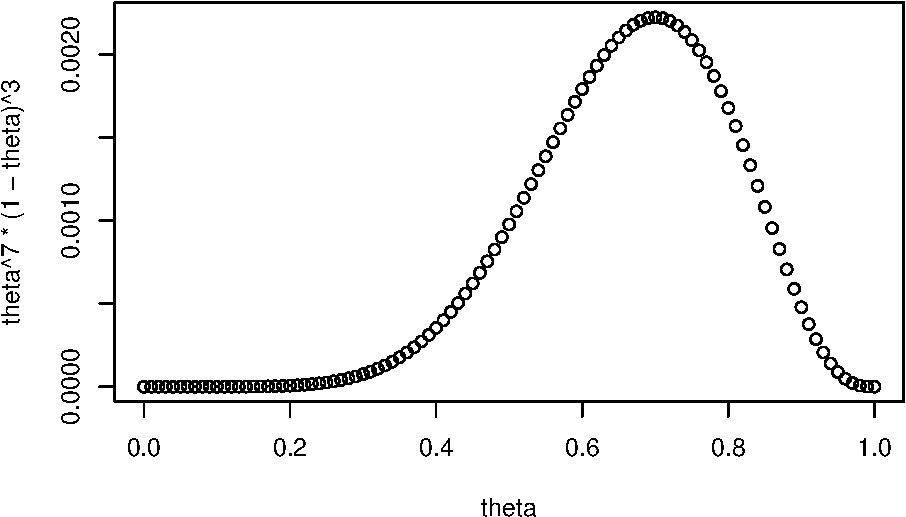
\includegraphics{_main_files/figure-latex/unnamed-chunk-3-1.pdf}

\begin{Shaded}
\begin{Highlighting}[]
\FunctionTok{cat}\NormalTok{(}\StringTok{"The maximum value of the distribution is:"}\NormalTok{ ,theta[}\FunctionTok{which.max}\NormalTok{(theta}\SpecialCharTok{\^{}}\DecValTok{7}\SpecialCharTok{*}\NormalTok{(}\DecValTok{1}\SpecialCharTok{{-}}\NormalTok{theta)}\SpecialCharTok{\^{}}\DecValTok{3}\NormalTok{)])}
\end{Highlighting}
\end{Shaded}

\begin{verbatim}
## The maximum value of the distribution is: 0.7
\end{verbatim}

Instead of having a known probability, we can work the other direction and calculate the most likely value for \(\theta\) given an observed data set. To keep things tractable, assume 10 flips, and we observe 7 heads. That is, \(L(\theta | \sum y_i=7, N=10)\) -- we may generate a value for \(\theta\) that maximizes the probability of observing 7/10 heads.

Formally,
\[L(\theta)=\Pi p(y_i | \theta)\].

Thus, the likelihood equation is the probability of observing \(y\) given some \textbf{best guess} of \(\theta\). Below, we'll very briefly develop a few techniques to formulate this guess

We've now observed the data, and instead of knowing \(\theta\), we can estimate the most plausible value of \(\theta\), considering our data. If we flip a coin ten times and observe seven heads, what is a value of \(\theta\) that is most likely to produce this sequence of results? It's 0.7; the maximum likelihood estimate of \(\theta\) is 0.7.

All the code does is take the probability of observing a head at each trial and multiplied these together. If we simulate values of \(\theta\), we find a single peaked function with a maximum value of 0.7.

In particular, we have identified a value of \(\theta\) in the population that was most likely to produce the observed data. In other words, we assume:

\[p(y|\theta)=\prod_{n=1}^Np(y_n|\theta)=\prod_{n=1}^N\theta^{y_n}(1-\theta)^{1-{y_n}}\]
(Bishop 2006, page 69).

If the sequence of results is \({H,H, T, H, T, T, T, T, T, T}\), if \(\theta=0.1\), then we multiply \(0.1 \times 0.1 \times 0.9 \times 0.1 \times 0.9^6\). By doing this for every value of \(\theta\), we want to find the highest probabilty associated with \(\theta\). This is precisely the logic of maximum likelihood: Observe a dataset and find a value of \(\theta\) that is most likely to have produced that dataset. What you can see is that the function is peaked. There is only one value that maximizes the ``likelihood function'\,' which is simply:

\begin{eqnarray}
p(y|\theta)=\prod_{n=1}^Np(y_n|\theta)=\prod_{n=1}^N\theta^{y_n}(1-\theta)^{1-{y_n}}
\end{eqnarray}

I've solved the problem with a simulation. In fact, that's not required. In this case, there is a closed form solution to the problem. In particular, we take the logarithm of the likelihood function, and solve by taking partial derivatives and setting these values to zero.

In this example, you've probably noticed that the maximum likelihood estimate for \(\theta\), given \(n\) Bernoulli trials is simply \(k/n\), where \(k=\sum y_i\). We'll rely on this logic throughout the semester -- and we'll extend this considerably -- but for now it's really just important to conceptually understand the motivation, which is to find the most likely value of \(\theta\) that produced the observed distribution of data.

As King (1998) notes, ``\textbf{Maximum Likelihood Estimation} is a theory of point estimation that derives in this very direct way from the likelihood function. The maximum is not always a very good summary of the entire likelihood function, but it is very convenient and often useful'' (p.~24)

\subsection{Bayesian Analysis}\label{bayesian-analysis}

This likely seemed like a really roundabout way to approach the obvious estimate of \(\theta\). Yet, often the likelihood equation (in this case the binomial) is not so simple. We're also left with a less than intuitive probability statement -- what is the value of \(\theta\) that maximized the probability of observing a set of observed heads? We're not really able to make a probablistic statement about \(\theta\) from the method. For instance, we cannot something like, ``based on the data, I am 90\% certain that its value lies between 0.6 and 0.7, which corresponds to the conclusion that the coin is unfair''!

But, we can invert the probability statement and model \(p(\theta|Y)\) by applying Bayes' rule.There are many good ways to acquaint onself with Bayesian analysis. By far the best (in my opinion), is the third edition Bayesian Data Analysis, which is a fantastic introduction to Bayesian analysis for the social sciences, written by Andrew Gelman and colleagues (Gelman, Carlin, Stern, Dunson, Vehtari and Rubin 2014). Unlike some of the alternatives, it presents a relatively useful balance of technical details and more practical considerations.\} In fact, Thomas Bayes (an English reverend and mathematician) and independently, Pierre LaPlace, thought about the problem somewhat differently, by focusing on \(\theta\) (Gelman, Carlin, Stern, Dunson, Vehtari and Rubin 2014).

We can't really make a probabilistic statement about \(\theta\); we can only find a value that is most likely to have produced a dataset. This is functionally equivalent to what you've learned about inference thus far. Probabilities don't allow us to make probabilistic statement about a parameter, rather, they pertain to a procedure. If I say, \textbf{The 95\% confidence interval around my estimates of a candidate's share of the New Hampshire Primary vote is {[}32, 36{]}, what does that mean?} Can I say, there is a 95\% chance that the true parameter is between 32 and 36? We could use Bayes' Rule to flip this logic on it's head. Instead of a confidence interval, let's just use \(pr(TrumpWins)=\theta\)\}

Let's just assume the following for \(Y={H, T, H, H, T}\). What is the \$pr(\theta \textbar{} Y \$. We already know the maximum likelihood estimator of \(\theta=0.60\) (why?). But recall, we also need to make a statement about \(p(Y)\) as well as \(p(\theta)\). We have a probability density for \(Y \sim binomial(Y, N, P)\). But, this density is multiplied by our ``prior beliefs'\,' about \(\theta\). There isn't sufficient space here to outline all the steps, but suffice it to say that because we must multiply two probability densities, it's more tractable if they are conjugate distributions. This simply means the posterior, the end result, is the drawn from the same family of PDFs as the prior.

\section{Quick Review}\label{quick-review}

\textbf{Correlated random variables}. If we have two independent random variables, \(x\) and \(y\), with means \(\mu_x\) and \(\mu_y\) and standard deviations, \(\sigma_x\) and \(\sigma_y\), then \(x+y\) yields \(\mu_x+\mu_y\). The standard deviation then is \(\sqrt{\sigma^2_x+\sigma^2_y+\rho\sigma_x\sigma_x}\), where \(\rho\) is the correlation between the variables (Gelman and Hill 2009, p.14). We often assume the two variables follow a multivariate normal distribution, \(z_k \sim N(\mu_k, \Sigma_{kk})\). \(\mu_k\) represents the means of the random variables, \(\Sigma\) represents a covariance matrix, with variances on the diagonal and covariances on the off diagonal.

\textbf{Variable Transformations}. Often, we transform variables (perhaps to restore normalcy). A common technique is to transform a variable by taking its natural logarithm. The exponential of the mean of these log values is called the geometric mean; the geometric standard deviation is the exponential of the standard deviation of logarithmic values. These are \emph{not} the means and standard deviations on the original scale, which are calculated as \(exp(\mu+0.5 \sigma^2)\) and \(exp(\mu+0.5 \sigma^2)\sqrt{exp(\sigma^2)-1}\), respectively (Gelman and Hill, p.15).

Moreover, if we have two independent variables, \(x\) and \(y\), with means \(\mu_x\) and \(\mu_y\) and standard deviations, \(\sigma_x\) and \(\sigma_y\), then \(x+y\) yields \(\mu_{x+y}\mu_x+\mu_y\). The standard deviation then is \(\sqrt{\sigma^2_x+\sigma^2_y+\rho\sigma_x\sigma_x}\) (Gelman and Hill 2009, p.14). We often assume the two variables follow a multivariate normal distribution, \(z_k \sim N(\mu_k, \Sigma_{kk})\). \(\mu\) represents the means of the random variables, \(\Sigma\) represents a covariance matrix, with variances on the diagonal and covariances on the off diagonal.

Recall the \textbf{central limit theorem} states that by drawing repeated samples and calculating the means, then the distribution of sample means will be approximately normal. A \emph{sampling model}, which we commonly work with, is a model applied to a sample from a population; we in turn use that model to make an inference about a population. In fact, a test-statistic or estimand is used in this model to draw an inference about a \textbf{population parameter}. Statistics are often called parameter estimates.

The \textbf{standard error} of a statistic represents uncertainty about the parameter estimate. In the case of a mean, recall that the central limit theorem allows us to estimate the standard deviation of sample means, \(\sigma/\sqrt{n}\). When dealing with proportions, the standard error is \(\sqrt{p(1-p)/n}\). Say we are interested in the difference between two proportions, we must then calculate the standard deviation of the differences, or \(\sqrt{sd_{p1}^2+sd_{p2}^2}\)

\textbf{The Expected Value}. The expected value is the ``average'\,' value over many draws -- it's useful to think of it from the perspective of frequentism. For a discrete distribution, then:

\[E(x_i)=\sum_{i}^{K} x_i p(x_i)\]

Again, this doesn't tell us anything about a single, or even predicted, \(x_i\) value. It is the value of \(x_i\), weighted by \(p(x_i)\). Take a simple example, flipping a coin. Let's say \(H=Y=1\), \(T=Y=0\). As such, if we flip a coin 10 times, then \(E(Y_i)=\sum y_i  f(y)=(0.5)^{10}\).\footnote{You may also write it as $E(x_i)=\sum_i^{K} x_i f(x_i)$.}

We have conceptually the same thing for a continuous variable, where

\[E(x)=\int_{-\infty}^{\infty}x f(x)dx\].

Again, it's simply the sum of the occurence weighted by the probability of that occurence. If \(y=f(x)=a+bx\), where \(a\) and \(b\) are simply constants, then \(E(y)=E(a+bx)=aEx+b\). The expected value of a fixed value or constant value is a constant. You should recognize this from the linear regression course, \(E(Y)=a+b\bar{X}\).

The expected value is also called the \emph{first moment} of a distribution.

\section{Properties of Estimators}\label{properties-of-estimators}

We're often concerned with making inferences about a population from a sample. Recall, in the frequentist tradition, we think of parameters as fixed characteristics of the population; statistics are derived from sample(s) drawn from the population. They are often qualified with some degree of uncertainty. An estimator is the formula or equation used to represent what we think is the process governing a parameter. So, \(y_i=\alpha+\beta x + \epsilon\) forms the relationship between x and y in the population, governed by fixed parameters \(\alpha\), \(\beta\), and an error term. This is not the estimator. The estimator is the method we then use to guess these parameters. Ordinary least squares is an estimator. It's one of many estimators. Much of POL 681 was oriented around showing it is the best linear unbiased estimator, in particular conditions.

The issue is that we only have a sample, or set of samples. Thus we wish to draw an inference about the population from the sample. The various properties of an estimator can be explored in several ways. One is to assume a sample is observed over repeated trials, so we have repeated samples. We could then perform our estimation procedure across samples and compile these estimates. Recall the logic of the central limit theorem, for instance.

If we were able to repeatedly draw samples and run our estimation procedure, we are left with a \textit{sampling distribution}. We can then explore properties of an estimator by examining this distribution. Most notably, the distribution will have mean

\[E(\hat {\theta})\]

\[var(\hat{\theta})=E(\hat{\theta}-E(\hat{\theta}))^2\]

With \(\sqrt{var(\hat{\theta})}\) as the standard deviation of the sampling distribution. We can then establish three statistics to explore the properties of an estimator. The \textbf{sampling error} is the deviation between our estimator \(\hat{\theta}\) and the population parameter (\(\theta\)). There will always be some degree of error by drawing a sample from a population. We may wish to minimize this sampling error, but we shouldn't expect it to be zero.

\textbf{Bias} is the difference between the expected value of an esimator relative to the true population parameter, i.e., \(\hat{\theta}-\theta\). Note how this is different from the sampling error. The sampling error refers to the difference for a single estimate produced from our estimator. Bias is the average of many samples analyzed with an estimator.

We're often also interested in how much an estimator varies about a true population parameter. Here, let's define the \textbf{Mean Squared Error} (MSE), or \(E(\hat{\theta}-\theta)^2\). Again, notice the difference here. Here, we are concerned with how much an estimator varies around the true population parameter. It can be shown that the MSE may be rewritten as

\[E(\hat{\theta}-E(\hat{\theta}))^2 +[E(\hat{\theta}-\theta)]^2\]

In other words, the MSE is a function of the variance of the estimator and the bias of the estimator. We generally wish for this value to be small. For instance, if we were to compare two estimators, we should prefer the estimator that is unbiased with minimum variance, which of course translates to having the smallest MSE.

\section{Finite Sample Properties}\label{finite-sample-properties}

Much of what you've learned in POL 681 pertained to OLS and \textbf{small sample properties}. Some estimators have desirable properties even when a sample is small. For instance, OLS has desirable small sample properties. When we refer to small sample properties, this typically entails.

Unbiasedness, or \(E(\hat{\theta})=\theta\). Over repeated samples, the mean of the sampling distribution will equal the true population parameter. Although it may seem that unbiaseness is sufficient to draw conclusions about an estimator, it's not. The reason is that it refers to repeated samples. We have no idea if a parameter estimate from a single sample is near to the true population value.

Efficiency, or

\[var(\hat{\theta})<var(\tilde{\theta})\].

Compared to other estimators, our estimator should have smaller variance.

In some cases, there is a tradeoff, in that we may have an estimator that is known to be biased, but it has smaller variance. Or, we have an estimator that is unbiased, but has huge variance. In fact, we can operationalize this further by simply using the MSE. We may prefer an estimator that has the smallest MSE, even if it's known to be biased.

An example of this is ridge regression. Recall, that in ridge regression, in some circumstances, we'll have an estimator with bias, but smaller variance -- it will have a lower MSE.

Something that we haven't sufficiently established yet is the large or asymptotic properties of an estimator. What happens to the behavior of the sampling distribution as the sample size approaches infinity.

\section{Asymptotic Properties}\label{asymptotic-properties}

These refer to the properties of an estimator as the sample size approaches infinity. In other words, as the sample size gets larger and larger, what happens to the characteristics of an estimator? An estimator is said to be \emph{asymptotically unbiased} if

\[\lim_{n\to\infty} E(\hat{\theta})=\theta\]

A perfect example of this is the estimate of the sample variance; you may recall that the population variance is:

\[\sigma^2={{1}\over{n}}(x-\mu_{x})^2\]

But the sample variance is:

\[\sigma^2={{1}\over{n-1}}(x-\bar{x})^2\]

But, the population variance is an unbiased estimator as the sample size increases. In particular,

\[\lim_{n\to\infty} E(\hat{\sigma^2})=\lim_{n\to\infty} [{{n-1}\over{n}}]\sigma^2=\sigma^2\]

Note that as n approaches infinity, the term \([{{n-1}\over{n}}]\) approaches 1 and the estimator converges to the population parameter.

An estimator is \emph{consistent} if:

\[P\lim_{n\to\infty}(|\hat{\theta}-\theta|<d)=1\]

then,

\[Plim_{n\to\infty}(\hat{\theta})=\theta\]

Really, this is subtly different from asymptotic unbiasedness. What it means is that the probability that the estimator is not different from the population parameter is 1 as the sample size approaches infinity. Put slightly different, the probability increases to 1 that as the sample size increases the estimator converges to the population parameter. It is possible -- in fact quite common -- for an estimator to be biased but consistent. We sometimes refer to this as the bias/variance tradeoff. A prime example is the variance estimate above. When we divide by \(n\) this is also called the MLE estimatate of the variance. It is biased in small samples, but consistent and asymptotically unbiased. I like to think of consistency more in terms of the variance of an estimator, such that \(P\lim_{n\to\infty}\) represents the point at which the variance is 0 and the entire distribution collapses to one value -- i.e., \(\lim_{n\to\infty} MSE(\hat{\theta}=0)\)

\subsection{The Bias Variance Tradeoff}\label{the-bias-variance-tradeoff}

By now, you should be intimately familiar with a traditional linear equation.

\[Y_i=\beta_0+\beta_1 x_{1,i}+\beta_2 x_{2,i}+\dots+\beta_k x_{k,i}+e_i\]

We can find these parameters by minimizing the residual sum of squares.

\[RSS=\sum_{i=1}^N=Y_i-(\beta_0+\beta_1 x_{1,i}+\beta_2 x_{2,i}+\dots+\beta_k x_{k,i})\]
A problem that often arises in practice is that of collinearity -- with finite samples, it is not uncommon to find that some variables are (imperfect) linear combinations of other variables, which doesn't necessarily affect the parameter estimates, but will grossly exaggerate the standard errors. What does this mean? We end up with an unbiased, but inefficient estimate. This is rarely ideal. First, we cannot effectively test hypotheses and second unless the model is strongly informed by theory, it is possible that we could drop a variable. Of course, we know that if we drop a variable that should be in the model, then we risk biased estimates. This is one issue that is very common in applied statistics; theory may not be terribly informative and it is unclear whether a variable should be included in the model. Plus, if we include irrelelevent variables, this will promote ``overfitting'' whereby our ``out-of-sample'' predictions (think election forecasting) will be off.

We'll encounter the so-called bias-variance tradeoff frequently in the class. Some estimators may be unbiased, but inefficient. This is a very real problem. Though unbiased sounds good, recall what it means: The expected value of the parameter estimate is the true population value. We approached it with relatively simple proofs -- recall, the Gauss-Markov theorem -- though we can also really easily see it in practice. Consider the following:

  \bibliography{book.bib,packages.bib}

\end{document}
